% Nota de coyuntura — Encuesta Intercensal 2025. Versión 1.0 (v0.2 + the four edits of the Anne/Cath v0.2 review).
% Build instructions: _crossrefs/_build_instructions/2026-09-23_DFD_nota-EIC2025_build-instruction.md (v0.1)
%                     _crossrefs/_build_instructions/2026-09-23_demographics_commit-endorsements_nota-v0.2.md (v0.2)
% v1.0 edits:         _crossrefs/corpus/demographics/_pending/2026-09-23_nota-EIC2025-v0.2_Anne-Cath-review.md §5
% Every number is \N{key}, generated by scripts/04_numbers.py from results/*.csv. Build with ./build.sh.
\documentclass[10pt,a4paper]{article}
\usepackage[T1]{fontenc}
\usepackage[utf8]{inputenc}
\usepackage{lmodern}
\usepackage[spanish,mexico]{babel}
\usepackage[a4paper,top=1.5cm,bottom=1.9cm,left=1.9cm,right=1.9cm,footskip=0.9cm]{geometry}
\usepackage{microtype}
\usepackage{graphicx}
\usepackage{booktabs}
\usepackage{xcolor}
\usepackage[font=small,labelfont=bf,labelsep=period,skip=3pt]{caption}
\usepackage{enumitem}
\usepackage{fancyhdr}
\usepackage[hidelinks,pdftitle={México después de la Encuesta Intercensal 2025},
  pdfauthor={Héctor J. Villarreal Páez},
  pdfsubject={Nota de coyuntura, versión 1.0 (pendiente de firma)},
  pdfkeywords={build_instruction: _crossrefs/_build_instructions/2026-09-23_demographics_commit-endorsements_nota-v0.2.md}]{hyperref}

\input{build/numbers.tex}

\definecolor{ink2}{HTML}{52514E}
\definecolor{boxbg}{HTML}{F4F3EF}
\definecolor{draft}{HTML}{B3261E}

\setlength{\parindent}{0pt}
\setlength{\parskip}{4pt}
\setlist{nosep,leftmargin=1.2em}
\renewcommand{\arraystretch}{1.12}
\captionsetup[figure]{name=Figura}
\captionsetup[table]{name=Cuadro}

\pagestyle{fancy}
\fancyhf{}
\renewcommand{\headrulewidth}{0pt}
\fancyfoot[L]{\scriptsize\color{ink2}ITED · Escuela de Gobierno y Transformación Pública, Tecnológico de Monterrey · septiembre de 2026 · versión 1.0}
\fancyfoot[R]{\scriptsize\color{ink2}\thepage/3}

\newcommand{\sect}[1]{\par\vspace{3pt}{\large\bfseries #1}\par\vspace{1pt}}
\newcommand{\sub}[1]{\textbf{#1}\enspace}
\newsavebox{\recbox}
\newenvironment{recuadro}[1]
  {\par\vspace{2pt}\noindent\begin{lrbox}{\recbox}\begin{minipage}{\dimexpr\linewidth-2\fboxsep\relax}
   \setlength{\parskip}{2pt}\textbf{#1}\par}
  {\end{minipage}\end{lrbox}\colorbox{boxbg}{\usebox{\recbox}}\par\vspace{2pt}}
\newcommand{\borrador}{\textcolor{draft}{\scriptsize\textsc{[borrador para edición]}}}

\begin{document}

% ============================================================ PÁGINA 1
{\small\color{ink2}Nota de coyuntura · versión 1.0 · pendiente de firma\par}
\vspace{2pt}
{\LARGE\bfseries México después de la Encuesta Intercensal 2025: menos nacimientos, una ventana fiscal más corta\par}
\vspace{3pt}
{\normalsize Héctor Juan Villarreal Páez · ITED, Tecnológico de Monterrey\quad\borrador\par}
\vspace{6pt}

La Encuesta Intercensal 2025 (EIC) del Instituto Nacional de Estadística y Geografía (INEGI) contó
\N{eicPob} millones de habitantes. Estimó una tasa global de fecundidad (TGF, el número de hijos
que tendría una mujer a lo largo de su vida) de \N{eicTgf} en 2024; con el mismo método, el Censo
de 2020 la había estimado en \N{censoTgf} para 2019. La edad mediana es de \N{eicEdadMediana} años
y el \N{eicSesentaycincoPct}\,\% de la población tiene 65 años o más: uno de cada diez. Entre 2020
y 2025 emigraron \N{eicEmigrantes} millones de personas y regresaron \N{eicRetornos} mil.

\begin{figure}[h]
\centering
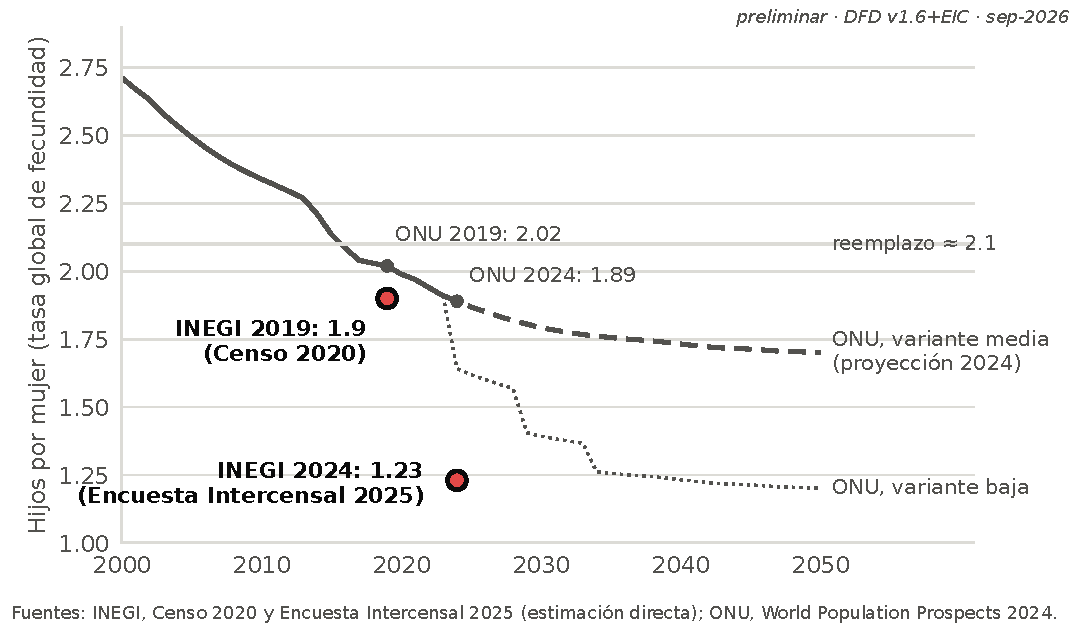
\includegraphics[width=0.97\linewidth]{figures/F1_fecundidad_inegi_vs_onu.pdf}
\caption{Fecundidad observada por el INEGI frente a la proyección de la Organización de las
Naciones Unidas (ONU). La ONU suponía \N{onuTgfDosmilveinticuatro} hijos por mujer para 2024; el
INEGI midió \N{eicTgf}. Lo observado ya está en el piso de largo plazo de la variante baja de la ONU.}
\end{figure}

\begin{recuadro}{Recuadro 1. Lo que cambió}
\begin{itemize}
\item La proyección de la ONU (\emph{World Population Prospects} 2024, variante media) suponía una
  TGF de \N{onuTgfDosmilveinticuatro} para 2024. La observada es \N{eicTgf}.
\item La variante baja de la ONU supone \N{onuBajaDosmilveinticuatro} para 2024 y llega a
  \N{onuBajaDosmilcincuenta} hacia 2050; lo observado (\N{eicTgf}) ya está en el piso de largo plazo
  de esa variante.
\item Los niños que no nacieron ya no están en la estructura por edad. La Encuesta cuenta cerca de
  \N{gapNinos} millones de menores de 15 años menos que los que supone la proyección oficial del
  Consejo Nacional de Población (CONAPO) para 2025.
\end{itemize}
\end{recuadro}

\newpage
% ============================================================ PÁGINA 2
\sect{Cuatro escenarios, 2025--2050}
Un escenario no es un pronóstico: responde a la pregunta «¿qué pasaría si la fecundidad se
mantuviera en este nivel?». Los cuatro parten de la población observada por la Encuesta y comparten
mortalidad y migración; difieren en la fecundidad. \emph{Optimista} reproduce el supuesto de la ONU
(de \N{onuTgfDosmilveinticinco} en 2025 a \N{onuTgfDosmilcincuenta} en 2050). \emph{Central}, con
\N{centralTgf} hijos por mujer, era el escenario base de este proyecto antes de la Encuesta.
\emph{INEGI directo} mantiene constante el nivel observado, \N{inegiTgf}. \emph{Estrés} supone que
la caída sigue hasta \N{estresPiso} en \N{estresAnio}.

\begin{figure}[h]
\centering
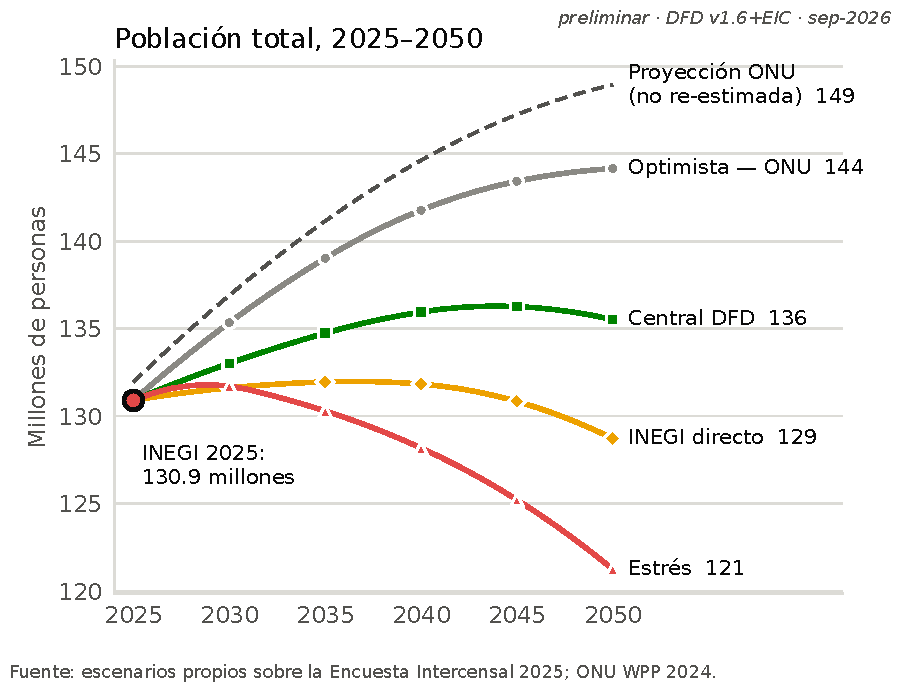
\includegraphics[height=5.05cm]{figures/F2_poblacion_total.pdf}\hfill
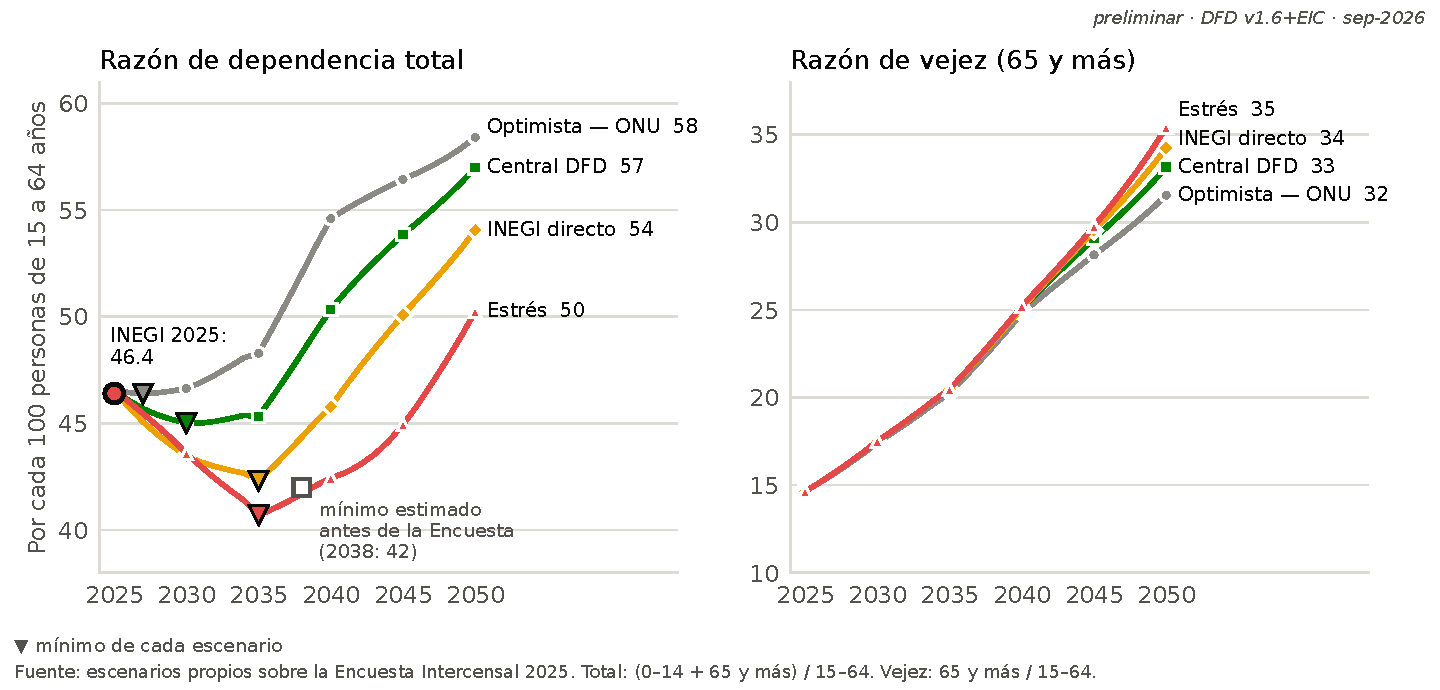
\includegraphics[height=5.05cm]{figures/F3_razon_dependencia.pdf}
\caption{Izquierda: población total. Centro: razón de dependencia total, personas de 0 a 14 y de 65
años o más por cada 100 de 15 a 64. Derecha: razón de vejez, personas de 65 años o más por cada 100
de 15 a 64. La razón total casi no baja porque la caída de niños compensa el aumento de adultos
mayores (en Central, entre 2025 y 2035, de \N{ydr2025} a \N{ydr2035_central} niños y de
\N{oadr2025_central} a \N{oadr2035_central} adultos mayores por cada 100 en edad de trabajar); el
costo fiscal de un adulto mayor es mayor que el de un niño.}
\end{figure}

\begin{table}[h]
\centering\small
\begin{tabular}{lccccc}
\toprule
\multicolumn{6}{r}{\scriptsize\color{ink2}preliminar}\\
Escenario & TGF supuesta & Población 2050 & \multicolumn{2}{c}{Razón de dependencia mínima} & Razón de vejez\\
          &              & (millones)     & año & valor & 2050\\
\midrule
Optimista --- ONU & \N{onuTgfDosmilveinticinco}\,$\to$\,\N{onuTgfDosmilcincuenta} & \N{pob2050_optimista} & \N{tdrMinAnio_optimista} & \N{tdrMin_optimista} & \N{oadr2050_optimista}\\
Central           & \N{centralTgf} & \N{pob2050_central} & \N{tdrMinAnio_central} & \N{tdrMin_central} & \N{oadr2050_central}\\
INEGI directo     & \N{inegiTgf}   & \N{pob2050_inegi}   & \N{tdrMinAnio_inegi}   & \N{tdrMin_inegi}   & \N{oadr2050_inegi}\\
Estrés            & \N{centralTgf}\,$\to$\,\N{estresPiso} & \N{pob2050_estres} & \N{tdrMinAnio_estres} & \N{tdrMin_estres} & \N{oadr2050_estres}\\
\midrule
\multicolumn{2}{l}{\color{ink2}Proyección ONU (referencia, no re-estimada)} & \color{ink2}\N{onuPobDosmilcincuenta} & & & \\
\bottomrule
\end{tabular}
\end{table}

\begin{recuadro}{Recuadro 2. Supuestos y estado de los resultados}
\scriptsize
\begin{itemize}
\item \textbf{Base de población.} Encuesta Intercensal 2025 (\N{eicPob} millones, incluida la población
  complementaria), trasladada de octubre a mitad de 2025 con sus propios componentes observados.
  La EIC cuenta \N{chkEic} millones de personas de 65 años y más. El censo de 2020, envejecido cinco
  años, da \N{chkCenso} millones, y la conciliación del CONAPO, \N{chkConapoOct}. La diferencia se
  concentra entre los 65 y 69 años y se revisará con los microdatos de la EIC. Con la cifra más baja, la
  cotización de equilibrio de 2025 sería \N{tauSensDif2025} puntos menor; la de 2050, sólo
  \N{tauSensDif2050}.
\item \textbf{Mortalidad.} Tasas por edad y sexo de la Conciliación Demográfica y Proyecciones de
  Población del CONAPO (2023), 2025--2050.
\item \textbf{Migración.} Salida neta de \N{migEic} mil personas al año hasta 2030 (Encuesta
  Intercensal 2020--2025; es una cota inferior, porque no capta hogares que emigraron completos), que
  se reduce linealmente a \N{migTaper} mil en 2040 (rango 2015--2020: \N{migRangoLo}--\N{migRangoHi}
  mil) y se mantiene; con la estructura por edad y sexo de los emigrantes que midió la Encuesta
  (\N{migHombresPct}\,\% hombres). En Estrés no se reduce; en Optimista se usa la migración de la ONU.
\item \textbf{Fecundidad.} Las cuatro trayectorias descritas, con el patrón por edad del CONAPO para
  2024. La TGF intercensal es una estimación directa y puede subestimar el nivel.
\item \textbf{Ventana.} El texto reporta el año y el nivel del mínimo de la razón de dependencia. Si se
  quiere un periodo: en Central la razón está a menos de un punto de su mínimo entre
  \N{spanIni_central} y \N{spanFin_central}.
\item \textbf{Pensiones.} Cotización de equilibrio ilustrativa $\tau=\rho\cdot$(razón de vejez)$/e$, con
  $\rho=\N{rho}$ (tasa de reemplazo del modelo fiscal del proyecto) y $e=\N{eEmpleo}$, la tasa de empleo
  de 15 a 64 años (INEGI, Encuesta Nacional de Ocupación y Empleo, \N{enoeTrim}), constante.
\item \textbf{Modelo.} Proyección por componentes, por sexo y edad simple, anual (proyecto DFD,
  instrucciones de escenarios v1.6). El modelo fiscal estructural del proyecto (IM-6, OLG) no se
  re-ejecutó para esta nota; los indicadores fiscales son aritmética sobre los escenarios.
\item \textbf{Estado.} Resultados preliminares, versión 1.0. La versión de registro es el reporte
  trimestral Q4-2026.
\end{itemize}
\end{recuadro}

\newpage
% ============================================================ PÁGINA 3
\sect{Consecuencias fiscales}
\sub{La ventana de reforma ya está abierta.} En el escenario Central el mínimo de la razón de
dependencia llega hacia \N{tdrMinAnio_central} en \N{tdrMin_central}, no hacia \N{qTresMinAnio} en
\N{qTresMin} como estimaba este proyecto antes de la Encuesta. La razón hoy es \N{eicTdr} (Encuesta
Intercensal 2025): entre hoy y su mínimo sólo baja \N{tdrBaja} puntos. Medido así, el bono demográfico
está prácticamente agotado. Con la fecundidad observada (INEGI directo) el mínimo es \N{tdrMin_inegi}
en \N{tdrMinAnio_inegi}. La entrada a la ventana puede rezagarse hasta un paso de proyección.

\sub{Pensiones: la aritmética de un sistema de reparto.} En un sistema estilizado en que los
cotizantes de hoy pagan las pensiones de hoy y la tasa de reemplazo ($\rho$, pensión media como
fracción del ingreso laboral medio) está fija, la cotización de equilibrio es $\rho$ por el número de
personas de 65 años o más por cada persona de 15 a 64, dividido entre la tasa de empleo ($e$). El
cálculo es ilustrativo y no representa a ningún sistema existente.

\begin{table}[h]
\centering\small
\begin{tabular}{lccc}
\toprule
Cotización de equilibrio (\% del salario), $\rho=\N{rho}$, $e=\N{eEmpleo}$ & 2025 & 2035 & 2050\\
\midrule
Central        & \N{tau2025_central} & \N{tau2035_central} & \N{tau2050_central}\\
INEGI directo  & \N{tau2025_inegi}   & \N{tau2035_inegi}   & \N{tau2050_inegi}\\
\color{ink2}Central, con la población de 65 y más del CONAPO & \color{ink2}\N{tauSens2025_central} & \color{ink2}\N{tauSens2035_central} & \color{ink2}\N{tauSens2050_central}\\
\bottomrule
\end{tabular}
\end{table}
\vspace{-6pt}
Esta cotización es una referencia: la aportación, sobre los ingresos de todos los trabajadores, que
financiaría una pensión igual a la mitad del salario en un sistema de reparto. No es la tasa de ningún
régimen vigente. Hasta 2035 la cotización no depende de la fecundidad: la aritmética de pensiones de la próxima década
ya la escribieron quienes están vivos. Mantener la tasa de reemplazo exige que la cotización pase de
\N{tau2025_central}\,\% a \N{tau2050_central}\,\% (Central) o \N{tau2050_inegi}\,\% (INEGI directo) en 2050.

\sub{Educación: cohortes que ya nacieron.} Entre 2025 y \N{escolarAnioFijo} la población de 6 a 14
años baja de \N{escolar2025_central} a \N{escolar2031_central} millones (\N{escolarCambio2031_central}\,\%)
en todos los escenarios, cualquiera que sea la fecundidad: \N{escolarNacidosPts} puntos corresponden a
niños que ya nacieron y \N{escolarEmigraPts} a la emigración de familias. Después depende de ella: en 2050 serían \N{escolar2050_central} millones en Central
y \N{escolar2050_inegi} en INEGI directo (\N{escolarCambio2050_central}\,\% y
\N{escolarCambio2050_inegi}\,\%). La caída de la matrícula básica de aquí a \N{escolarAnioFijo} ya
ocurrió.

\sub{Crecimiento: la aritmética.} El producto crece por la productividad de cada trabajador y por el
número de trabajadores. La población de 15 a 64 años crece \N{glA_central}\,\% anual entre 2025 y 2035
y empieza a caer en \N{glNeg_central} en los cuatro escenarios, porque esas personas ya nacieron; entre
2035 y 2050 cae \N{glB_central}\,\% anual en Central y \N{glB_inegi}\,\% en INEGI directo. La deuda y
las pensiones se pagan con el producto total, no con el producto per cápita.

\begin{figure}[h]
\centering
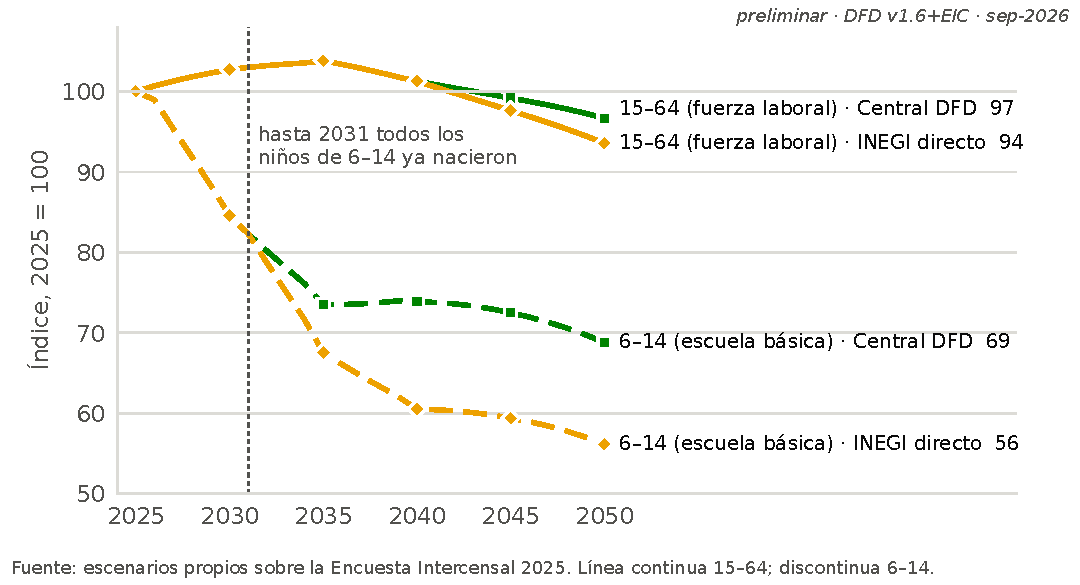
\includegraphics[width=0.66\linewidth]{figures/F4_dos_cohortes.pdf}
\caption{Dos cohortes que ya nacieron: población de 6 a 14 años (escuela básica) y de 15 a 64
(fuerza laboral), índice 2025\,=\,100.}
\end{figure}

\vspace{-4pt}
\sub{Tres implicaciones} \borrador
\begin{enumerate}
\item La reforma que se pensaba para finales de la década de 2030 tiene su ventana en la primera mitad.
\item El gasto educativo puede reasignarse hacia calidad y primera infancia sin recortar cobertura,
  porque la matrícula cae por sí sola.
\item Ampliar la formalidad alivia la cuenta sólo mientras los nuevos cotizantes no se jubilan; en el
  largo plazo, con reemplazo fijo, la cotización depende de la razón de vejez y de la tasa de empleo.
\end{enumerate}

Lo que puede cambiar este panorama: las estadísticas vitales definitivas de 2025 del INEGI, la
proyección del CONAPO re-basada en la Encuesta y los microdatos de la Encuesta (INEGI, noviembre de 2026).

{\scriptsize\color{ink2}\textbf{Fuentes.} INEGI, Encuesta Intercensal 2025, Reporte de Resultados 37/26 y
datos abiertos; INEGI, Censo de Población y Vivienda 2020; INEGI, Encuesta Nacional de Ocupación y Empleo,
microdatos, \N{enoeTrim}; ONU, \emph{World Population Prospects} 2024 (población, fecundidad, variantes
media y baja); CONAPO, Conciliación Demográfica 1950--2019 y Proyecciones de la Población de México
2020--2070 (2023); Fernández-Villaverde y Norrick (2026), «Terra Incognita», \emph{Annual Review of
Economics} (en prensa), para el contraste entre niveles y razones y la crítica metodológica a la ONU;
instrucciones de escenarios DFD v1.6.\par}

\end{document}
